\subsection{Hardware - V1.0}

This version of the battery module is working completely different than the later versions. 
It was intended to be a rough prototype for the base module V1.0 \& V1.1 to test the 
concept of a pluggable battery module. The battery module is used to power the basic node,
without the need to connect a USB-C cable.

    \subsubsection{Module-Connector}
        The battery module is connected to the following voltages:

        \begin{itemize}
            \item 1. 3V3 - The battery module powers the basic node over this pin
            \item 2. VBUS - used to charge and disable the battery module when USB is connected
            \item 3. $V\_BAT$ - used to monitor the battery voltage
            \item 4. EN-MODUL - Used to disable the linear voltage regulator on the basic node
            \item 5. GND - Ground
        \end{itemize}

        \begin{figure}[H]
            \centering
            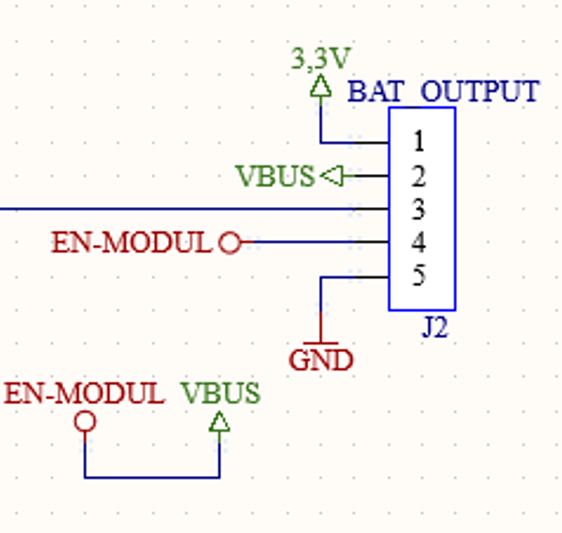
\includegraphics[width=0.4\textwidth]{assets/HW/BatteryV1-Connector-schematic.png}
            \caption{Battery implemented in the schematic.}
        \end{figure}
        
        With the voltages the basic node is powered and the battery is charged.

    \subsubsection{Battery}

    \subsubsection{DC-DC-Converter}

        A buck-boost converter is used to convert the 3.7V from the battery to 3.3V to power the
        basic module. The used IC is the TPS63001 from Texas Instruments it is a high efficiency
        buck-boost converter with a 96\% efficiency. The inductor and the output voltage were
        calculated like stated in the datasheet\cite{}. The inductor was selected by calculating
        the maximum inductor current:

        \begin{equation}
            D = \frac{V_{OUT} - V_{IN} }{V_{VOUT}}
        \end{equation}

        \begin{equation}
            I_{PEAK} = \frac{I_{OUT}}{\eta \cdot (1 - D)} + \frac{V_{IN} \cdot D}{2 \cdot f \cdot L} 
        \end{equation}

        The output voltage was set with a resistor divider to 3.3V:

        \begin{equation}
            R1 = R_2 \cdot (\frac{V_{OUT}}{V_{FB}} - 1)
        \end{equation}

        \begin{figure}[H]
            \centering
            
\includegraphics[width=0.4\textwidth]{assets/HW/TBD2.png}
            \caption{DC-DC-Converter implemented in the schematic.}
        \end{figure}

        There were problems with getting the IC to work properly. 
    
    \subsubsection{PCB}
        The PCB of the battery module is a 2-layer board with the same size as the basic module
        with 35x70mm.

        \begin{figure}[H]
            \centering
            
\includegraphics[width=0.4\textwidth]{assets/HW/TBD2.png}
            \caption{Battery PCB.}
        \end{figure}